\subsection{\href{http://www.nanocut.com/}{nanocut}}
   \hypertarget{subsec:nanocut}
   Para la firma nanocut de Moldavia, se desarrolló un controlador de motor \textit{permanent
   magnet synchronous motor} (PMSM) utilizando una placa de desarrollo de Texas Instruments con un microcontrolador de tiempo real de la linea C2000 sobre la cual se desarrollaron los algoritmos de control de torque, velocidad y posición a lazo cerrados utilizando un encoder óptico relativo.\\
   Se logró poner en marcha un prototipo que sera la base de hardware y firmware para un nuevo driver genérico de motores para las máquinas CNC que cuenta dicha empresa. \\
   Se utilizó un método de control vectorial FOC, y se implementaron las transformadas de Clarke/Parke y varios PID's anidados para lograr los objetivos con la máxima performance. \\
   En la figura \ref{fig:nanocut_electronica} se pueden ver las herramientas de hardware y los algoritmos implementados en funcionamiento.\\
     \begin{figure}
      \begin{center}
         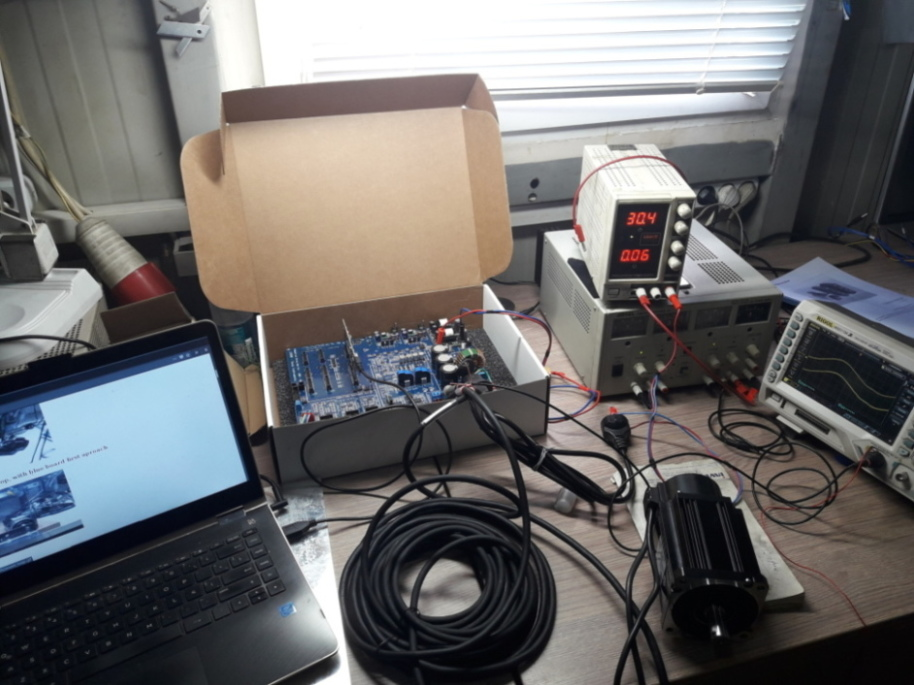
\includegraphics[width=0.3\textwidth]{portfolio/nanocut1.jpg}
         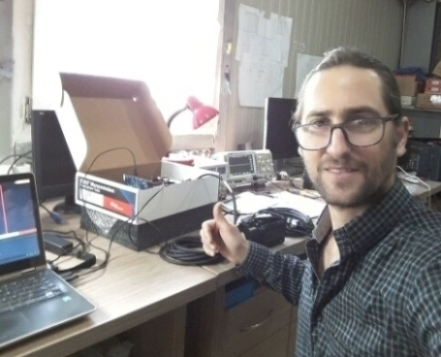
\includegraphics[width=0.3\textwidth]{portfolio/nanocut2.jpg}
         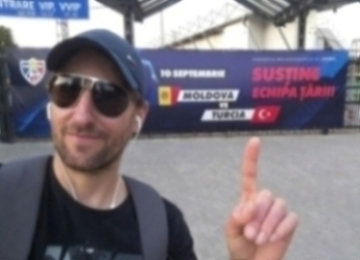
\includegraphics[width=0.3\textwidth]{portfolio/nanocut3.jpg}
      \end{center}
      \caption{Herramientas de desarrollo y captura de resultados de los algoritmos para el control de un motor PMSM}
      \label{fig:nanocut_electronica}
   \end{figure}
   En la figura \ref{fig:nanocut_mecanica} se muestra el prototipo funcionando en los laboratorios de Moldavia.
  \begin{figure}
      \begin{center}
         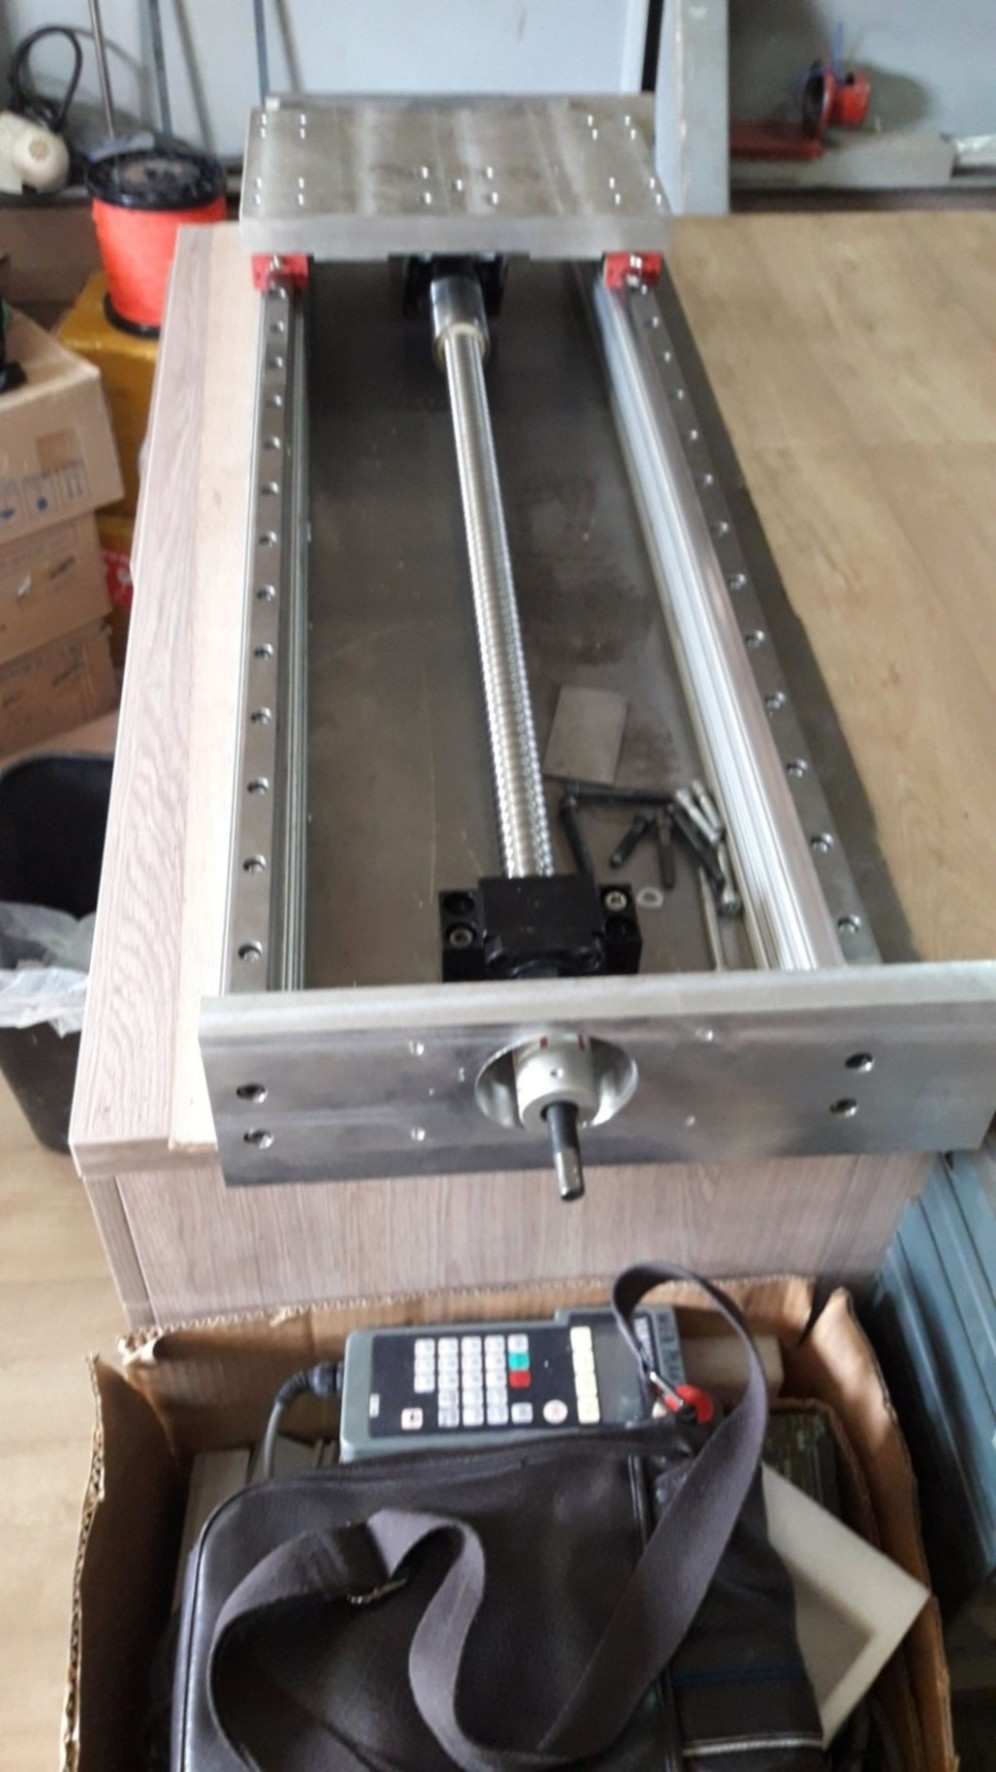
\includegraphics[width=0.3\textwidth]{portfolio/nanocut4.jpg}
         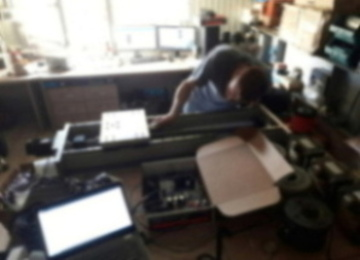
\includegraphics[width=0.3\textwidth]{portfolio/nanocut5.jpg}
         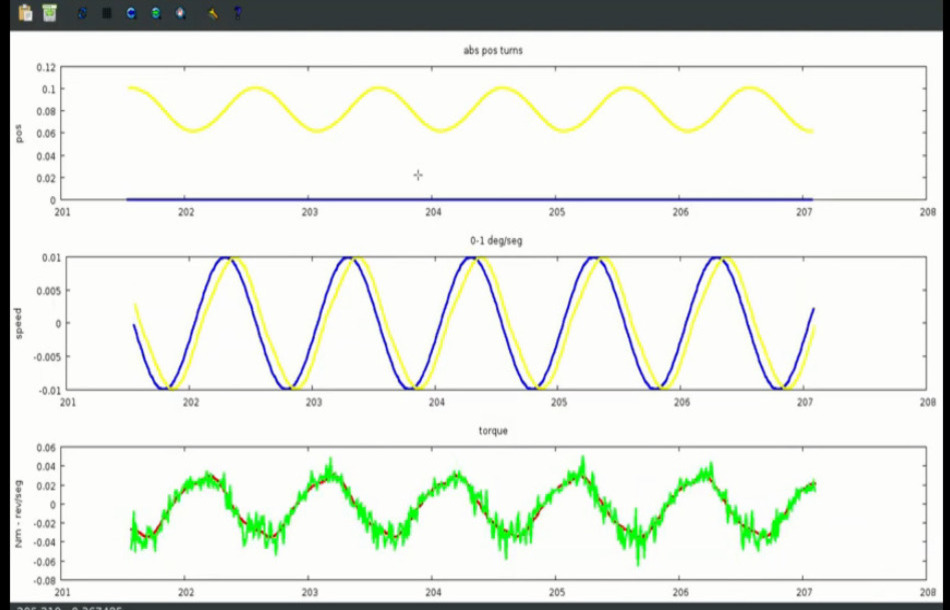
\includegraphics[width=0.3\textwidth]{portfolio/nanocut6.jpg}
      \end{center}
      \caption{Prototipo mecánico para las pruebas de los algoritmos de control de torque, velocidad y posición utilizando un motor PMSM}
      \label{fig:nanocut_mecanica}
   \end{figure}

